\section{Fundamentação Teórica}

No presente trabalho, valeu-se de filtros IIR para resolução de uma situação problema que exigia a minimização de ruído em um sinal dado, com frequência fundamental de 60hz. Para tanto, valemo-nos de diferentes modelos (a saber, Butterworth, Chebyshev tipo I e II, e Elíptico), alterando os parâmetros julgados relevantes de modo a minimizar o erro frente ao sinal original, ponderando pelo impacto computacional que a solução traria.

Em relação aos algoritmos avaliados, temos também particularidades teóricas em seu funcionamento, conforme explicitado em \cite{oppenheim2009} que podem explicar a adequação (ou não) à situação presente. Em comum, todos são filtros digitais passa baixa, atuando de modo a retirar as frequências indesejadas introduzidas no ruído. No entanto, há divergências de funcionamento, particularmente em relação à velocidade e suavidade de transição nas diferentes bandas do sinal, e consequentemente no ripple acarretado.

Para o filtro Butterworth, temos que sua resposta em magnitude é monotônica, tanto na banda de aceitação quanto de corte, ou seja, não introduz ripple, sendo uma opção de filtro bem suave. Conforme aumentamos a ordem, no entanto, é observado um comportamento mais brusco de transição

Já os filtros de Chebyshev aceitam a existência de ripple, mas apenas em uma das bandas, seja na de aceitação , mantendo a banda de rejeição monotônica (tipo I); Ou na de rejeição, mantendo a banda de aceitação plana (tipo II). Apesar de indesejado, a introdução do ripple pode ser útil visto que tem como consequência uma transição consideravelmente mais rápida que filtros monotônicos, como Butterworth

Por fim, o filtro Elíptico permite existência de ripple em todo seu espectro, tanto na banda de aceitação quanto de rejeição. Isso torna sua transição bem agressiva, possuindo a faixa de transição mais rápida de todos, mas ocasionando em um erro distribuído maior.


\begin{figure}[h]
\centering
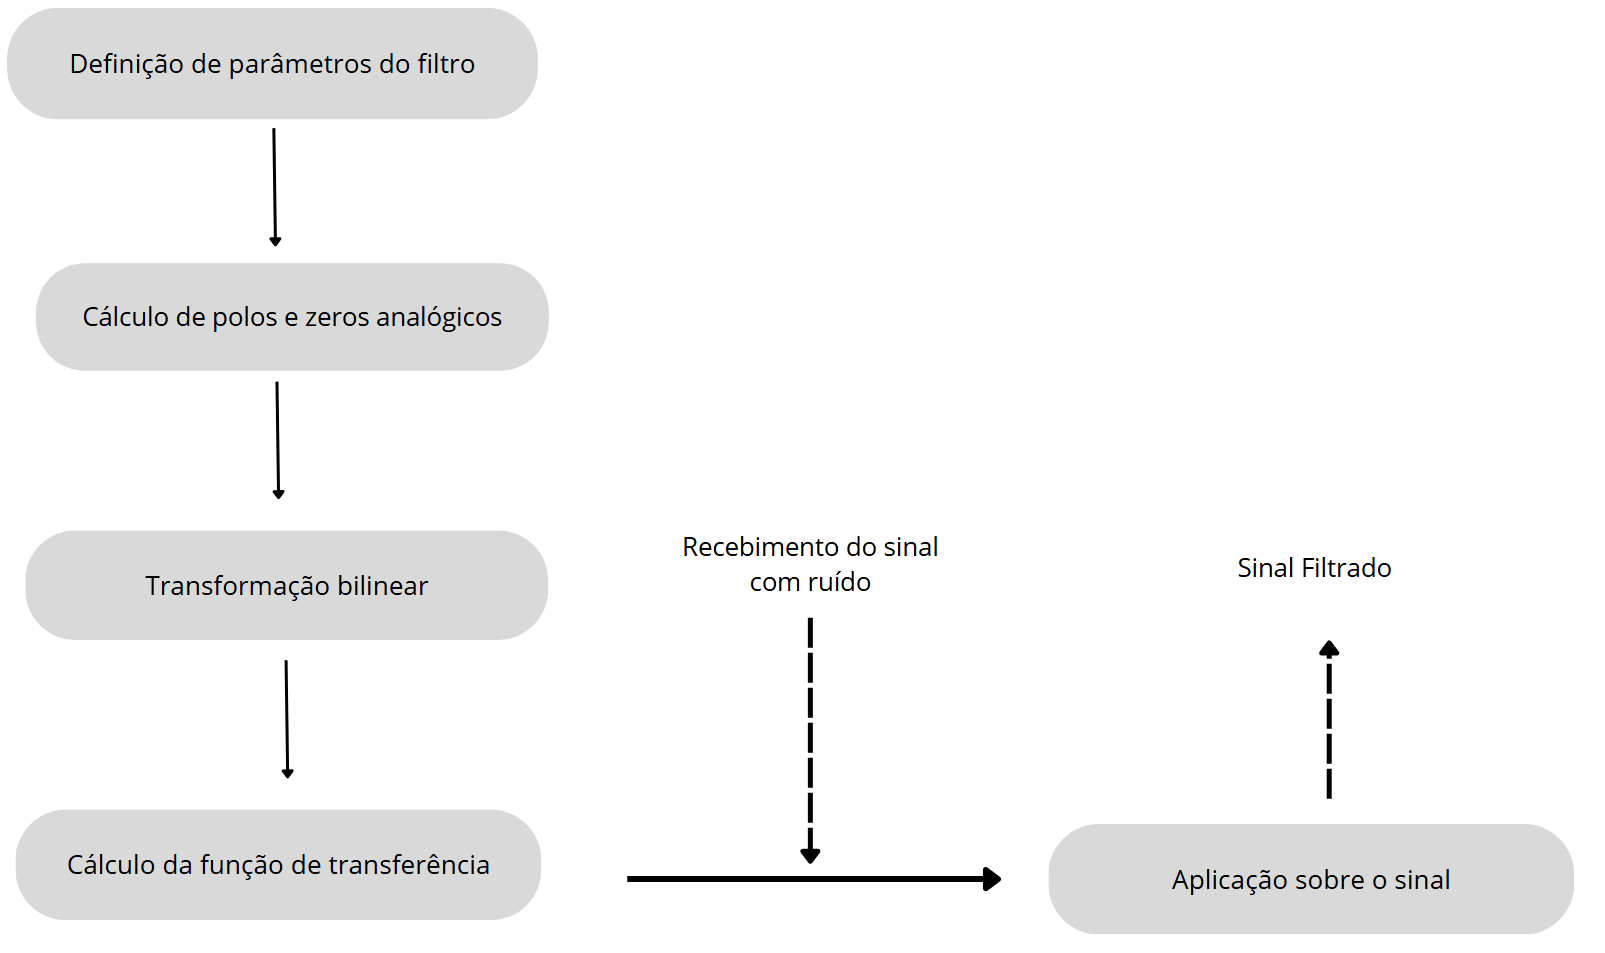
\includegraphics[width=0.45\textwidth]{Fluxograma.png}
\caption{Fluxograma do filtro de Chebyshev Tipo II}
\label{fig:flowchart}
\end{figure}

\subsection{Filtros IIR e Transformação Bilinear}
Um filtro IIR é descrito por uma equação de diferenças recursiva~\cite{oppenheim2009},
cuja função de transferência no domínio~$z$ é uma razão de polinômios:
\begin{equation}
H(z) = \frac{\sum_{k=0}^{M} b_k\,z^{-k}}{1 + \sum_{k=1}^{N} a_k\,z^{-k}}.
\label{eq:Hz}
\end{equation}
A recursividade (presença de polos) permite obter respostas seletivas com ordens
baixas, ao custo de exigir verificação de estabilidade: todos os polos devem
estar no interior do círculo unitário, $|p_i| < 1$. O projeto parte de um
protótipo analógico passa-baixas, mapeado para o domínio discreto pela
\emph{transformação bilinear}
\begin{equation}
s = \frac{2}{T}\,\frac{1 - z^{-1}}{1 + z^{-1}},
\end{equation}
que preserva a estabilidade, mas introduz distorção de frequência
(\emph{warping}), compensada por pré-distorção (\emph{prewarping}) na frequência
de corte. As rotinas utilizadas executam esse procedimento internamente.

\subsection{Filtragem Causal versus Fase Zero}
A filtragem direta (\emph{causal}) introduz atraso de fase dependente da
frequência, deformando a forma de onda. Em processamento \emph{offline}, a
filtragem de \textbf{fase zero} aplica o filtro duas vezes, nos sentidos direto e
reverso, cancelando o atraso de fase e dobrando a atenuação efetiva~\cite{gustafsson}.
Ambas as estratégias foram avaliadas: a causal por funcionar em tempo real e a de
fase zero por ter melhor desempenho \emph{offline}.

\subsection{Realização em Seções de Segunda Ordem (SOS)}
Para ordens elevadas, a forma direta~\eqref{eq:Hz} é numericamente mal
condicionada: o erro de arredondamento dos coeficientes pode levar à
instabilidade. Por isso adotou-se a realização em \textbf{seções de segunda
ordem} (cascata de biquads), bem mais robusta e de uso comum na prática.

\subsection{Métricas de Avaliação}
A qualidade da filtragem é medida pelo \textbf{erro quadrático médio}
\begin{equation}
\mathrm{RMSE} = \sqrt{\frac{1}{L}\sum_{n=0}^{L-1}
\bigl(x[n] - \hat{x}[n]\bigr)^2},
\label{eq:rmse}
\end{equation}
onde $x$ é o sinal de referência e $\hat{x}$ o sinal filtrado. Complementarmente,
o \textbf{ganho de relação sinal-ruído} (SNR) quantifica a melhoria em decibéis:
\begin{equation}
\Delta\mathrm{SNR} = 10\log_{10}\!\frac{\sum x^2}{\sum (\hat{x}-x)^2}
                   - 10\log_{10}\!\frac{\sum x^2}{\sum (x_{\text{ruído}}-x)^2}.
\label{eq:snr}
\end{equation}

\subsection{Implementação da Função de Filtragem}
A filtragem foi implementada em Python (bibliotecas \texttt{numpy} e
\texttt{scipy.signal}~\cite{scipy}) como uma função genérica, aplicável a qualquer
comprimento de sinal:

\begin{lstlisting}
def aplicar_filtro_iir(sinal, fs, f_corte, ordem,
                       tipo='butter', rp=0.5, rs=40.0,
                       fase_zero=True):
    Wn = f_corte / (0.5 * fs)
    sos = projetar_sos(tipo, ordem, Wn, rp, rs)
    if fase_zero:
        return signal.sosfiltfilt(sos, sinal), sos
    return signal.sosfilt(sos, sinal), sos
\end{lstlisting}

O projeto retorna os coeficientes em formato SOS; a filtragem de fase zero usa
\texttt{sosfiltfilt} e a causal, \texttt{sosfilt}. A frequência de corte é
normalizada pela frequência de Nyquist ($f_s/2$). Cabe ressaltar que o
significado de $f_c$ depende da aproximação: no Butterworth corresponde ao ponto
de \SI{-3}{\decibel}; no Chebyshev~I e no elíptico, à borda da banda de passagem
(onde termina a ondulação $r_p$); e no Chebyshev~II, à borda da banda de
\emph{rejeição} (onde a atenuação atinge $r_s$). Assim, o valor
$f_c=\SI{2700}{\hertz}$ do Chebyshev~II selecionado marca o início da banda de
rejeição, com a banda de passagem efetiva situada em frequência inferior.

\subsection{Busca em Grade e Critério de Estabilidade}
Para determinar os parâmetros ótimos, varreu-se uma grade de
\begin{itemize}
  \item \textbf{tipo}: \{Butterworth, Chebyshev~I, Chebyshev~II, elíptico\};
  \item \textbf{ordem}: de~1 a~8;
  \item \textbf{frequência de corte}: de \SI{300}{\hertz} a \SI{3300}{\hertz},
        em passos de \SI{100}{\hertz};
  \item \textbf{ondulação de passagem} $r_p$ (Chebyshev~I e elíptico):
        \{0{,}1;\ 0{,}5;\ 1{,}0\}~dB;
  \item \textbf{atenuação de rejeição} $r_s$ (Chebyshev~II e elíptico):
        \{30;\ 40;\ 50;\ 60\}~dB;
  \item \textbf{método}: fase zero e causal.
\end{itemize}
Vale uma observação sobre o enunciado, que pede testar diferentes
\emph{ordens} e \emph{janelamentos}. O janelamento é um parâmetro de projeto de
filtros FIR (resposta finita ao impulso), em que a resposta ao impulso
é truncada por uma janela como Hamming, Hann ou Kaiser; em filtros IIR ele não se
aplica, porque o filtro vem de um protótipo analógico mapeado para o
domínio discreto. O
parâmetro equivalente, que molda o formato da resposta, é o par
ondulação/atenuação ($r_p$, $r_s$); por isso a grade o varre
junto com tipo, ordem e frequência de corte.

Cada configuração foi submetida a uma verificação de estabilidade (todos os
polos com $|p_i|<1$, obtidos de \texttt{sos2zpk}). Como o projeto parte de
protótipos analógicos mapeados pela transformação bilinear, que preserva a
estabilidade, todas as \num{9920} configurações da grade resultaram estáveis;
elas foram então ordenadas pelo RMSE da Eq.~\eqref{eq:rmse}.

\subsection{Avaliação do Custo Computacional}
O custo foi medido cronometrando o processo completo (projeto dos
coeficientes mais filtragem) e tomando a \textbf{mediana} de \num{50}
execuções, o que reduz a influência das variações do sistema operacional. Depois
variou-se a ordem do filtro, com tipo e corte fixos, para ver o
compromisso entre RMSE e tempo de execução.
